% !TEX encoding = UTF-8
% !TEX program = pdflatex
% !TeX spellcheck = en_GB
% !BIB = biber

\documentclass[english]{article}
\usepackage{amsmath}
\usepackage{wasysym}
\usepackage{amssymb}
\usepackage{babel}
\usepackage[utf8]{inputenc}
\usepackage{graphicx}
\usepackage[obeyspaces]{url}
\graphicspath{{./images/}}
\usepackage{hyperref}
\hypersetup{
    colorlinks=true, 
	linkcolor=blue, 
	filecolor=blue, 
	citecolor = black,       
	urlcolor=blue, 
}
\usepackage{listings}
\lstset{
  xleftmargin=15pt,
  xrightmargin=0pt,
  framexleftmargin=0pt,
  framexrightmargin=0pt,
  basicstyle={\fontsize{9pt}{10pt}\ttfamily},
  columns=flexible,
  numbers=left,
  numbersep=10pt,
  numberstyle={\fontsize{9pt}{11pt}\selectfont\color[rgb]{0.4,0.4,0.1}},
  keepspaces=true,
  showstringspaces=false,
  identifierstyle=\color[rgb]{0.1,0.1,0.1},
  keywordstyle=\color{blue},
  commentstyle=\color[rgb]{0,0.3,0},
  morekeywords={rule, lemma},
  morekeywords=[2]{let, in},
  morekeywords=[3]{Fr, pk},
  morekeywords=[4]{In, Out},
  morekeywords=[5]{senc, aenc, h}
  morecomment=[s][keywordstyle3]{/*}{/},
  keywordstyle=\color[rgb]{0.44,0.57,0.65},
  stringstyle=\color{green},
  keywordstyle=[2]{\color[rgb]{0.86,0.57,0.18}},
  keywordstyle=[3]{\bfseries\color[rgb]{0,0.3,0.2}}
  }
\usepackage{biblatex}
\addbibresource{thud.bib}

\title{Small project - notes}
\author{Zanolin Lorenzo}

\begin{document}

\maketitle

\tableofcontents
\newpage

% scaletta:
% UWB, spiegazione generica di come funziona
% UWB analisi sulla sicurezza implementata da Apple
% FindMy spiegazione dell'architettura
% FindMy spiego ogni singola funzionalità
% FindMy esempio di come viene localizzato un oggetto (U1-uwb and BLE)
% AirTag analisi della sicurezza
% AirTag analisi caso stalking e come ovviare il problema
% AirTag esempio di funzionamento
% AirTag possibili utilizzi futuri

\begin{abstract}
  The main goal of this project is to dig into how Apple AirTags work, including their setup, security measures, and uses; since everything is tied to the FindMy network, we will also look into the security methods used in this network. The idea is to get a clear picture of how Apple AirTags are put together, how secure they are, and the different ways they're used in the FindMy network.
\end{abstract}

\section{Introduction}
In the rapidly evolving landscape of technological advancements, Apple's AirTags have emerged as a noteworthy innovation, offering a seamless solution to tracking and locating personal belongings. This paper delves into the architecture and security of AirTags, with a particular emphasis on the Ultra-Wideband (UWB) technology that underlies their functionality. Moreover, as AirTags operate within the framework of the FindMy network, this exploration extends to a thorough analysis of the security measures embedded in both the device and the overarching network; by unraveling the synergy between AirTags, UWB, and FindMy security, this paper aims to contribute insights into the robustness of the technological ecosystem that facilitates precise location tracking while addressing potential concerns surrounding privacy and data security.

In Section \ref{sec:uwb} we will explain some basics of UWB technology, continuing in Section \ref{sec:find} delving into the FindMy network analysis. Next we will deeply analyze the AirTag concept in \ref{sec:at}, concluding with some future uses.

\section{UWB}\label{sec:uwb}
\subsection{Overview}
In the realm of wireless communication technologies, Ultra-Wideband (UWB) stands out as a revolutionary paradigm, redefining the capabilities and applications of wireless connectivity. UWB operates by employing extremely low-power, short-duration pulses that span a broad spectrum, allowing for high data transfer rates and precise positioning capabilities. Originally conceived for military and radar applications, UWB has gradually permeated diverse sectors, finding particular prominence in consumer electronics, healthcare, automotive systems, and the Internet of Things (IoT).

The unique feature of UWB is its capacity to send information across a large frequency range, usually several gigahertz; a UWB transmitter sends billions of radio pulses across the wide spectrum frequency and a UWB receiver then translates the pulses into data. The shorter the duration of the impulse, the more precise the distance measurement will be. UWB achieves real-time accuracy because as it sends up to 1 billion pulses per second. Because of its wide spectrum utilization, UWB can coexist peacefully with other wireless technologies and send out massive volumes of data quickly.  Since its ability to transmit info across a wide radio bandwidth, from 500MHz to several gigahertz, this technology has a short range of operation. According to \cite{di2006uwb}, due to the low energy density and the pseudo-random (PR) characteristics of the transmitted signal, the UWB signal is noise-like which makes unintended detection difficult. By sending pulses in patterns, UWB encodes information and it takes between 32 and 128 pulses to encode a single bit of data, but given how fast the bits arrive, that enables data rates of 7 to 27 megabits per second. To increase UWB’s range and reception reliability, a \textit{MIMO} (multiple-input and multiple-output), distributed antenna system has been added to the standard that enables short-range networks. The antennas can be embedded into a smartphone or other devices such as a wristband or smart key.

According to \cite{aps}, Apple-designed U1 chip uses Ultra Wideband technology for spatial awareness— allowing iPhone 11, iPhone 11 Pro, and iPhone 11 Pro Max or later iPhone models to precisely locate other U1-equipped Apple devices.
When two U1 devices come close to eachother, the two start measuring their exact distance. The ranging is accomplished through Time of Flight (ToF), which is the time it takes for a pulse to get from point A to point B. According to IEEE 802.15.4a \cite{5394030}, UWB can determine the relative position of other devices in the line of sight even up to 200 meters.

A difference w.r.t. Bluetooth Low Energy is that with Bluetooth you can’t really measure location or distance. What you can do is to detect if a device like a smartphone is within a range of another device. Ultra-Wideband, in comparison, provides a much higher accuracy (up to a few centimeters). In contrast to Bluetooth Low Energy, the distance it measures is not based on the signal strength, but the time it takes the signal to travel from point A (smartphone) to point B (UWB tag). The following table represent the principal differences between the two technologies:

\begin{table}[h]
  \begin{tabular}{l|l|l|}
  \cline{2-3}
  {}                               & {\textbf{UWB}}                & { \textbf{Bluetooth (BLE Beacons)}} \\ \hline
  \multicolumn{1}{|l|}{{  \textbf{Battery}}}  & {  Low consumption}             & {  Low consumption}                  \\ \hline
  \multicolumn{1}{|l|}{{  \textbf{Range}}}    & {  up to 200 meters (656 feet)} & {  up to 70 meters (230 feet)}       \\ \hline
  \multicolumn{1}{|l|}{{  \textbf{Accuracy}}} & {  10 centimeters (3.9 inches)} & {  up to a meter}                    \\ \hline
  \multicolumn{1}{|l|}{{  \textbf{Cost}}}     & {  Low}                         & {  Low}                              \\ \hline
  \end{tabular}
  \end{table}

\subsection{Security analysis}
The fact that UWB pulses are resistant to the multipath effect\footnote{Multipath interference occurs when a signal from a transmitter arrives at a receiver via two or more routes; typically there is a direct path plus a number of indirect paths caused by reflections} is one of its key characteristics. This occurs when radio waves are reflected or refracted by artificial or natural objects near to the primary signal channel, causing the signal to reach the receiver via many paths. Positioning accuracy is improved by immunity to the multipath effect, particularly when compared to other technologies that are more vulnerable. Moreover, UWB's resilience to jamming and narrowband fading makes it a particularly reliable technology choice, even when several UWB systems are being used at once.

Another important aspect to consider is the resistance from Relay Attacks, which is a vulnerability of the majority of signals-based architectures. Within this attacks, the goal is to trick a car into thinking the key and owner are close by using two people with hacking devices. The first relays signals from the car to the second thief, who transmits the signal to the house. The key responds, allowing entry into the car. The relay attack intercepts and amplifies wireless signals used to unlock the door and start the car, despite the key's distance. With UWB that would not be possible due to its working scheme: to ensure the car doesn't have to make assumptions, rapid measurements are utilized to establish distance very precisely. Any attempt to relay attack or intercept the UWB signal will merely cause the answering device's acknowledgement signals to arrive later, indicating to the UWB-based lock and ignition that the responding device is actually farther away rather than closer. The car's presumption is replaced with assurance when using UWB, which greatly increases the security of the passive keyless entry system.

The implemented security measures, taken by Apple, are the following: MAC address randomization and frame sequence number randomization \cite{aps}.
%approfondisci meglio guardando nel dettaglio il payload di un pacchetto

\subsubsection*{MAC address randomization}
Apple platforms use a randomized media access control address (MAC address) when performing scans when not associated with another device. Because a device’s MAC address changes when disconnected from another device, it can’t be used to persistently track a device by passive observers of traffic.

\subsubsection*{Frame sequence number randomization}
Apple devices randomize the sequence numbers whenever a MAC address is changed to a new randomized address.

\section{FindMy network}\label{sec:find}
\subsection{Overview}
Apple created the sophisticated and extensive location-tracking technology, known as the FindMy network, which is intended to assist consumers in finding their compatible third-party accessories, such as Apple AirTags, as well as their Apple devices, including iPhones, iPads, Macs, and AirPods. By utilizing a blend of Ultra-Wideband (UWB) and Bluetooth Low Energy (BLE) technologies, the FindMy network facilitates accurate and instantaneous location tracking.

Because it may be used to find everything you need to find, Apple combined the Find My Friends and Find My iPhone apps into a single app that is simply called \textit{Find My}. Subsequently, Apple has consistently enhanced the Find My app, incorporating functionalities such as monitoring when a iPhone is disconnected, when it is turned off, and when it has been wiped.

The app is organized into several sections, accessible by tapping the tabs at the bottom. On the left, you can find people, in the middle, you can find your own devices and items, such as AirTags, and Find My-enabled Bluetooth items; finally on the right there's a \textit{Me} tab with all of your settings and info, as we can see in Figure \ref{findmy2}.

There are several useful features within this app, as example:
\begin{itemize}
  \item \textit{Separation alerts}: designed to let you know if you leave an Apple device, a device attached to an AirTag, or a Find My-enabled third-party device behind.
  \item \textit{Locating friends and sharing location}: implemented to locate friends and family members that have shared their location with you. You can view their location using the \textit{People} tab within the Find My app.
  \item \textit{Locating devices without connection}: lets your lost devices be located even when not connected to WiFi or LTE by leveraging Bluetooth BLE and proximity to other nearby Apple devices. When your lost device is offline but close to another device, it's able to connect to that other device over Bluetooth and relay its location. We will come back on this\ldots
  % ovviamente se il bluetooth è off allora non è rilevabile, non basta avere il chip U1 alimentato
  \item \textit{Anti-stalking measures}: designed to let you know if there's a Bluetooth item near you. You will receive a notification when an unknown item is found and moving with you, so you can make sure no one slips an AirTag or other Find My Bluetooth device into your things to track you. We will also come back on this\ldots
  \item \textit{Precision finding}: takes advantage of the U1 chip within AirTags and the iPhone 13, iPhone 12 and iPhone 11 models. Apple's U1 chip uses ultra-wide band techology to precisely locate and communicate with other U1-equipped devices, enabling AirTags and iPhone 13/12/11 models to work together.
\end{itemize}

\begin{figure}[t]
	\centering
	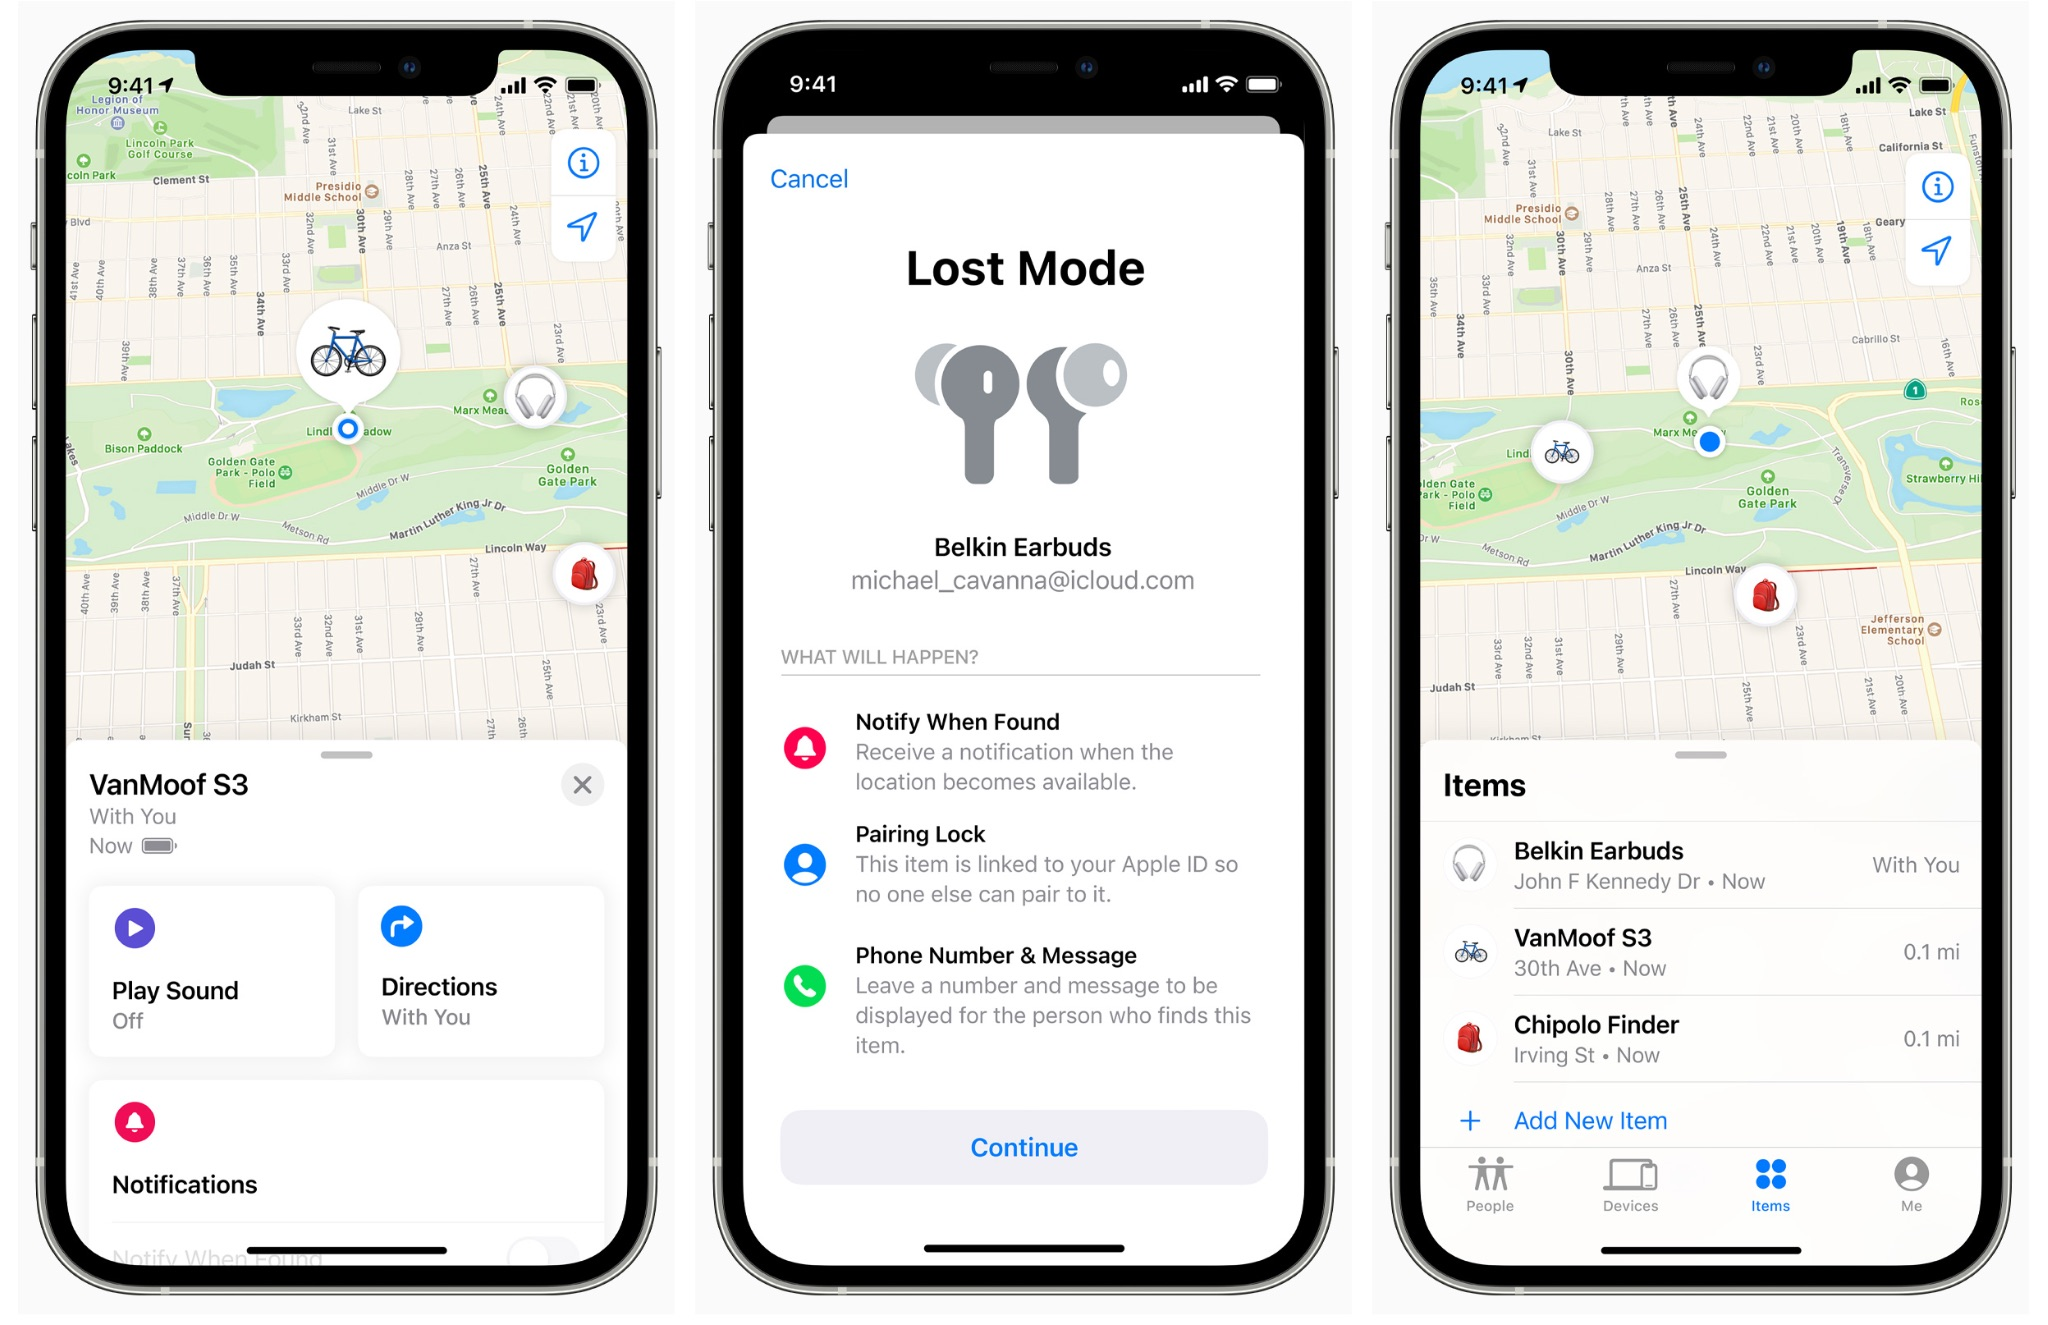
\includegraphics[width=.9\textwidth]{images/findmy.jpg}
	\caption{FindMy screenshots.}
	\label{findmy2}
\end{figure}

\subsection{Functioning}
As for the functioning, we will use the content of \cite{Mayo_2021,Itani_2021,Clover_2022,OBoyle_2021} to describe the entire process. First of all we want to register our products within the application; in case of a non-accessory item, it will automatically be inserted in the \textit{Devices} section. In case of accessories, like AirTag, you need to manually add them using the \textit{Items} section.

Now you should be able to localize online devices from the map; in case of a close AirTag you can also use the \textit{Precision finding} to locate the object using U1 chip (this function is only available for iPhone 11 and aboves), as represented in Figure \ref{findmy1}. The technology fuses input from the iPhone's camera, ARKit, accelerometer and gyroscope in order to guide the user to their AirTag using a combination of sound, haptics, and visual feedback. 

\begin{figure}[t]
	\centering
	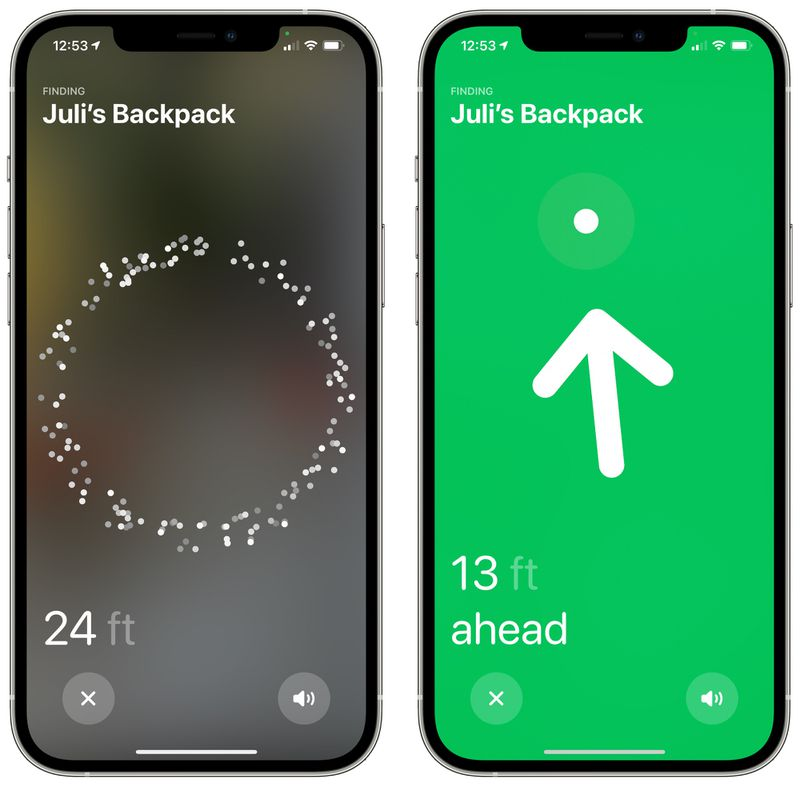
\includegraphics[width=.6\textwidth]{images/airtag-precision-finding-2.jpg}
	\caption{Precision Finding.}
	\label{findmy1}
\end{figure}

In case of a stolen device, you can always activate \textit{Lost Mode}; it will send you a notification as soon as the iphone is relevated, which means that if the phone will be connected to a network or via BLE to other Apple devices the owner will receive a message from FindMy containing the position of the device. Also, in this modality, all the registered cards in Apple Pay will be temporaneously disabled.

This technology seems already pretty useful, but if a device is powered off how can it be localized? With the introduction of iOS 15 and the U1 chips, Apple claimed that even a U1-based iPhone can be localized even when turned of if and only if the Bluetooth is turned on. From Apple: With iOS 15, your iPhone is still traceable through the Find My network even when the device is powered off. 
It seems that with iOS 15, the phone is not really fully powered off, it stays in a low-power state and acts like an AirTag, allowing any nearby iOS device to pick up the Bluetooth signal and send back its location.
This also means if the iPhone runs out of battery during the day, the owner still has a chance of finding its location for several more hours. In fact, Apple says the location tracking will even keep working whilst the phone is reset to factory settings with Activation Lock enabled. And what about other devices, like Macbooks? Since Apple has not commented on the matter, the author conducted some tests and discovered that, regrettably, even machines with high specifications lack the U1 chip and are therefore not localizable when turned off. 

As already written, AirTags can be tracked through the \textit{Items} tab and have all of the tracking features available to Apple devices like iPhones and iPads. There's a Lost Mode, and AirTags can also take advantage of the Find My network that allows them to be tracked by billions of iPhones, iPads, and Macs when they're out of range of the owner devices. The only way to stop an AirTag from being fully detectable is to remove the CR2032 coin battery (or when it fully discharges).

\subsection{Security analysis}
In this section we will analyze the security measures implemented in FindMy to increase the safety of the architecture. Let us add some more details in the process of localizing an object.
Let us first define a few terms in accordance with \cite{whocanfind}:
\begin{itemize}
  \item \textit{Owner Devices}: Owner devices share a common Apple ID and can use the Find My application on macOS, iOS and ipadOS to search for any devices of the same owner.
  \item \textit{Lost Devices}: Devices that determine to be in a lost state start sending out BLE advertisements with a public key to be discovered by finder devices. Apple devices are considered to be lost when they lose Internet connectivity. Third-party accessories \cite{gadget} are small battery-powered devices that can be attached to a personal item and are set up through an owner device. Accessories determine to be lost when they lose their BLE connection to the owner device.
  \item \textit{Finder Devices}: Finder devices form the core of the FindMy network. As of 2023, only iPhones and iPads with a GPS module are offering finder capabilities. Finder devices can discover lost devices and accessories by scanning for BLE advertisements. Upon receiving an advertisement, a finder creates an end-to-end encrypted location report that includes its current location and
  sends it to Apple’s servers. We will see what are the contents of the report.
  \item \textit{Apple’s Servers}: Apple’s servers store the location reports submitted by finder devices. Only owner devices can fetch those reports and decrypt them locally.
\end{itemize}
An online device can simply report its location to the user via iCloud. Find My works offline by sending out short range Bluetooth signals from the missing device that can be detected by other Apple devices in use nearby. Those nearby devices then relay the detected location of the missing device to iCloud so users can locate it in the Find My app while protecting the privacy and security of all the users involved. An example of the previous workflow is represented in figure \ref{process}.

\begin{figure}[]
	\centering
	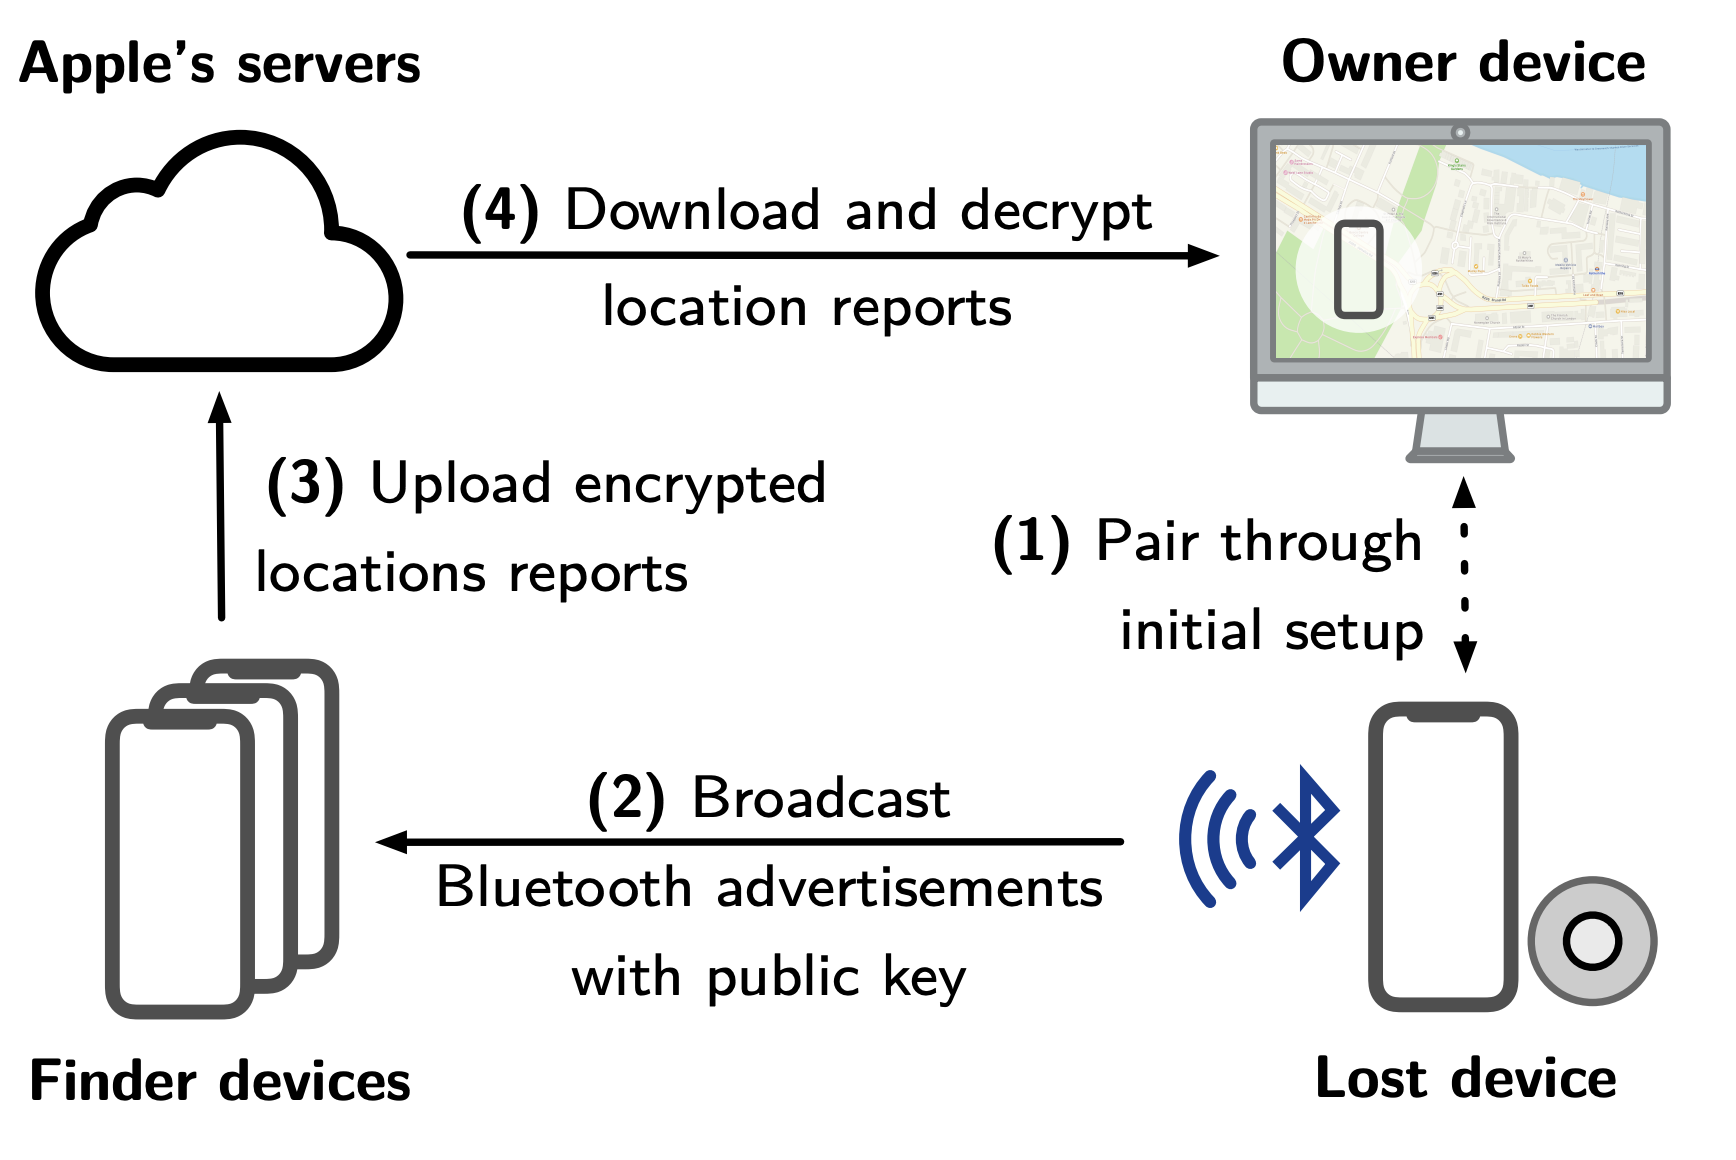
\includegraphics[width=.5\textwidth]{images/process.png}
	\caption{FindMy workflow (simplified).}
	\label{process}
\end{figure}

\begin{figure}[]
	\centering
	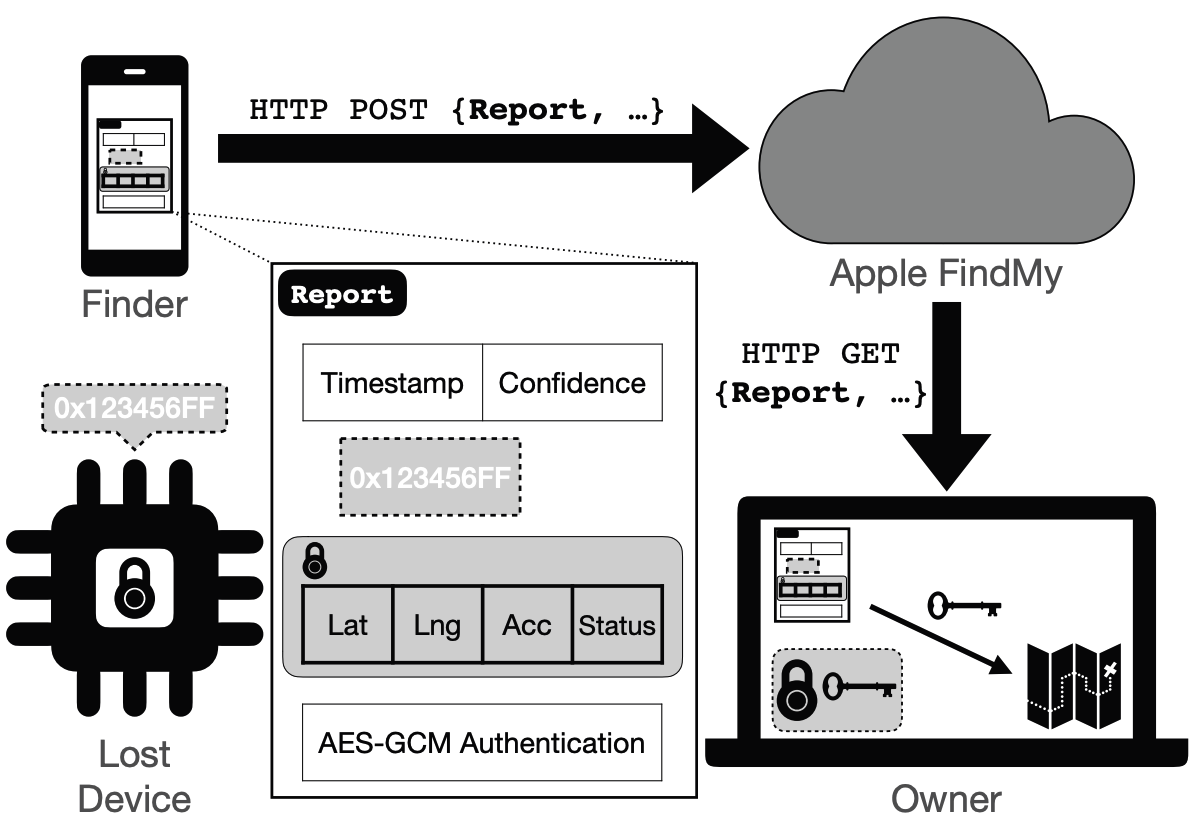
\includegraphics[width=.9\textwidth]{images/findmysec.png}
	\caption{Example of sent payload.}
	\label{findmy}
\end{figure}

We will now delve more in the used Cryptography protocols. 

\subsubsection{Advertisement keys}
FindMy utilises Elliptic Curves \cite{ec}; according to \cite{aps,whocanfind} the process to generate \textit{advertisement keys} is the following:
\begin{enumerate}
  \item Each owner device generates a private/public key pair
  $(d_0, p_0)$ on the NIST $P-224$ curve and a $32$-byte symmetric key $SK_0$ that together form the master beacon key. Those keys are never sent out via BLE and are used to derive the rolling advertisement keys included in the BLE advertisements. Note that device tracking is hard since rolling keys can be deterministically derived if and only if one knows the initial input keys $(d_0, p_0)$ and $SK0$.
  \item Advertisement keys $(d_i,p_i)$ are iteratively calculated as follows using the ANSI X.963 key derivation function $KDF$ \cite{ANSI} with $SHA-256$ \cite{sha} and a generator $G$ of the NIST P-224 curve:
  \begin{align}
    SK_i &= KDF(SK_{i-1},\ 'update',\ 32) \\
    (u_i, v_i) &= KDF(SK_i,\ 'diversify',\ 72) \\
    d_i &= (d_0 * u_i) + v_i \\
    p_i &= d_i * G
  \end{align}
  where Equation $(1)$ derives a new symmetric key from the last used symmetric key with 32 bytes length. Equation $(2)$ derives the so-called “anti-tracking” keys $u_i$ and $v_i$ from the new symmetric key with a length of $36$ bytes each. Finally, Eqs. $(3)$ and $(4)$ create the advertisement key pair via EC point multiplication using the anti-tracking keys and the master beacon key $d_0$.
\end{enumerate}

\subsubsection{Key synchronization}
To download and decode location information, the advertisement keys must be accessed by all owner devices. In order to synchronize the master beacon keys, FindMy uses iCloud to encrypt a property list file in the Galois/Counter mode of the Advanced Encryption Standard (AES-GCM) \cite{gcm}. The file's decryption key is kept in the iCloud keychain underneath the label “Beacon Store”.

\section{AirTag}\label{sec:at}

\printbibliography
\nocite{*}

\end{document}